%     AMS-LaTeX v.2 template for use with amsart
%
%     Remove any commented or uncommented macros you do not use.
\documentclass{amsart}
\usepackage[notref,notcite]{showkeys}
\usepackage{extarrows}
\usepackage{tikz-cd}
\usetikzlibrary{matrix}


\newtheorem{theorem}{Theorem}[section]
\newtheorem*{theorem*}{Theorem}
\newtheorem{lemma}[theorem]{Lemma}
 \newtheorem{corollary}[theorem]{Corollary}
 \newtheorem{proposition}[theorem]{Proposition}
 \newtheorem*{mainthm*}{Main Theorem}

\theoremstyle{definition}
\newtheorem{definition}[theorem]{Definition}
\newtheorem{example}[theorem]{Example}
\newtheorem{xca}[theorem]{Exercise}
\newtheorem{observation}[theorem]{Observation}
\newtheorem{conjecture}[theorem]{Conjecture}

\theoremstyle{remark}
\newtheorem{remark}[theorem]{Remark}

\definecolor{alert}{rgb}{0.8,0,0.3}
\newcommand{\alert}[1]{%
	\marginpar{%
		\ifodd\value{page} \raggedright \else \raggedleft \fi
		\footnotesize{\textcolor{alert}{#1}}
	}
}

%\numberwithin{equation}{section}

%    Absolute value notation
\newcommand{\abs}[1]{\lvert#1\rvert}
\newcommand{\D}{\operatorname{D}}
\newcommand{\V}{\operatorname{V}}
%\newcommand{\Hess}{\operatorname{Hess}}
\newcommand{\dist}{\operatorname{dist}}
\newcommand{\Vol}{\operatorname{Vol}}
\newcommand{\sign}{\operatorname{sign}}
\newcommand{\Div}{\operatorname{div}}
\newcommand{\C}{\operatorname{Cap}}
\newcommand{\pC}{{\operatorname{Cap}}_{p}}
%\newcommand{\R}{\operatorname{R_{eff}}}
\newcommand{\gr}{\operatorname{grad}}
\newcommand{\tors}{\operatorname{\mathcal{A}_{1}}}
\newcommand{\erre}{\mathbb{R}}
\newcommand{\ese}{\mathbb{S}}
\newcommand{\Hp}{\mathbb{H}}
\newcommand{\Lmod}{\operatorname{L}}
\newcommand{\Nu}{\operatorname{\#}}
\newcommand{\Trans}{\operatorname{T}}
\newcommand{\pL}{{\operatorname{\Delta}}_{p}}
\newcommand{\pLM}{{\operatorname{\Delta}}_{p}^{M}}
\newcommand{\pLP}{{\operatorname{\Delta}}_{p}^{S}}
\newcommand{\pLK}{{\operatorname{\Delta}}_{p}^{\mathbb{K}^{m,b}}}
\newcommand{\pCap}{{\operatorname{Cap}}_{p}}
\newcommand{\loc}{{\rm loc}}
%\newcommand{\k}{\operatorname{\mathbb{K}^{m}(b)}}
\newcommand{\Sup}{\operatorname{Sup}}
\newcommand{\Inf}{\operatorname{Inf}}
\def\kan{I\!\!K^n(b)}
\def\kal{I\!\!K^{n-1}(b)}
\def\kam{I\!\!K^m(b)}
\def\Han{\mathbb{H}^n(b)}
\newcommand{\Om}{\Omega}
\newcommand{\Sg}{\Sigma}
\newcommand{\ptl}{\partial}

\begin{document}

\title[Measure Concentration]{Measure concentration for compact and minimal submanifolds of the Sphere}



%    Remove any unused author tags.

%    author one information

%    author two information
\author{Vicent Gimeno i Garcia}
\address{Department of Mathematics, Universitat Jaume I-IMAC,   E-12071, 
Castell\'{o}, Spain}
%\curraddr{}
\email{gimenov@mat.uji.es}
\author{Vicente Palmer}
\address{Department of Mathematics, Universitat Jaume I-INIT,   E-12071, 
Castell\'{o}, Spain}
%\curraddr{}
\email{palmer@mat.uji.es}

\thanks{Research partially supported by  the Universitat Jaume I Research Program Project P1-1B2012-18, AEI-MINECO grant (FEDER) MTM2013-48371-C2-2-PDGI from Spanish Ministerio de Ciencia e Inovaci\'{o}n (MCINN), and by Generalitat Valenciana AICO/2021/2523}


\subjclass[2010]{Primary 58C40, 35P15, (53A10)}

\keywords{ measure concentration, isometric immersion, mean curvature, minimal submanifold}

%\date{\today}

\dedicatory{}



%%%%%%%%%%%%%%%%%%
%Abstract
%%%%%%%%%%%%%%%%%%%%
\begin{abstract}\textcolor{red}{V3.2}
Inspired by the equatorial concentration of measure phenomenon in the sphere $\ese^n(1)$, a result which is deduced from the general, (and intrinsic), concentration of measure in the sphere result presented by V. Milman and G. Schechtman in the lecture notes \cite{MS}, we describe in this paper an extrinsic equatorial concentration of measure satisfied by the closed, (compact without boundary), and minimal submanifolds $\Sigma^m$ isometrically immersed in the sphere $\ese^n(1)$.v3.\end{abstract}

\maketitle

%%%%%%%%%%%%%%%%%%
%Section: Introduction
%%%%%%%%%%%%%%%%%%%%
\section{Introduction}\label{sec:intro}\
%%%%%%%%%%%%%%%%%%%%%%

The deep connection between the notions of measure of sets, (in its meaning of Riemannian volume), distance between points and dimension in a Riemannian manifold is illustrated by the concentration of intrinsic measure phenomenon in the sphere as it was presented  by V. Milman and G. Schechtman in the lecture notes \cite{MS}.

In our opinion, an interesting question that can be raised from this result appears when considering it from an extrinsic point of view, that is, from the point of view of the submanifold theory. In this way, we are going to present a new notion of \lq\lq extrinsic equatorial measure concentration"  for submanifolds in the sphere, taking as a starting point the description of the intrinsic version of this phenomenon.  

The way to do that , as we shall see in this introduction, is based in the following idea:  from the general  concentration of intrinsic measure phenomenon it can be deduced an intrinsic equatorial measure concentration property satisfied by the strips around the equators of the sphere, which can be roughly described by saying that for ``very large" dimension, almost all measure in the sphere concentrates in these strips surrounding its equators. 

Then, this property shall be used in its turn to introduce  the concept of \lq\lq extrinsic equatorial measure concentration"  for submanifolds in the sphere above mentioned: we shall study the relative volume of the intersection of a closed and minimal submanifold with the above mentioned strips around the equators of the ambient sphere, concluding, as in the intrinsic case, that for \lq\lq very large" dimension, almost all measure in the submanifold concentrates in their intersection with the  strips surrounding its equators. 

In the lecture notes by V. Milman and G. Schechtman \cite{MS} we can find the following concentration of (intrinsic) measure phenomenon in the sphere $\mathbb{S}^n(1)$:

\begin{theorem}[Measure Concentration in the Sphere]\label{measurecon} If $A\subset \mathbb{S}^n(1)$ is a domain with ${\rm vol }(A)\geq \frac{1}{2} {\rm vol}(\mathbb{S}^n(1))$ then, for all $\epsilon \in [0,\frac{\pi}{2}]$, the  $\epsilon$-fattening of $A$ satisfies the inequality
\begin{equation}\label{eq1}
1 \geq \frac{{\rm vol}(A_\epsilon)}{{\rm vol}(\mathbb{S}^n(1))}\geq 1-\sqrt{\frac{\pi}{8}}e^{-\epsilon^2(n-1)/2}
\end{equation}
\noindent and hence, for all $\epsilon \in [0,\frac{\pi}{2}]$, 
\begin{equation}\label{eq2}
\lim_{n\to \infty} \frac{{\rm vol}(A_\epsilon)}{{\rm vol}(\mathbb{S}^n(1))}= 1.
\end{equation}
\end{theorem}  
Here, the $\epsilon$-fattening of $A$ is defined as
$$A_\epsilon:=\left\{x\in \mathbb{S}^n(1)\, :\, {\rm dist}^{\mathbb{S}^n(1)}(x,A)<\epsilon\, \right\}
$$
 
 This concentration of measure in the sphere is a consequence of the P. Levy's isoperimetric inequality,  which it is stated in \cite{MS} as follows:

 \begin{theorem}[Isoperimetric Inequality]\label{isopineq} For each $0<a<{\rm vol}(\mathbb{S}^n(1))$ and $\epsilon >0$,
$$
\min_{A\subset \mathbb{S}^n(1), {\rm vol}(A)=a}{\rm vol}(A_\epsilon)
$$
exists and it  is attained on the $\epsilon$-fattening $\left(B^{n,1}_{r(a)}\right)_\epsilon$ of any geodesic ball $B^{n,1}_{r(a)} \subset \mathbb{S}^n(1)$ such that
$$
{\rm vol}\left(B^{n,1}_{r(a)}\right)=a.
$$
\end{theorem}


  We are going to do some observations about how Theorem \ref{measurecon} comes from Theorem \ref{isopineq}. To see the idea behind  the proof of inequality (\ref{eq1}) we proceed in the following way: let us consider a  domain $A$ with ${\rm vol }(A)=a \geq \frac{1}{2} {\rm vol}(\mathbb{S}^n(1))$ and let us fix $\epsilon \in [0,\frac{\pi}{2}]$. Then,  applying Theorem \ref{isopineq}, and having into account that, fixed $\epsilon \in [0,\frac{\pi}{2}]$, the $\epsilon$-fattening of a geodesic ball $B^{n,1}_{r}$ is the ball $(B^{n,1}_{r})_{\epsilon}=B^{n,1}_{r+\epsilon}$, for all $r \in [0,\pi/2-\epsilon)$, it is easy to obtain the inequality
  
  $${\rm vol}(A_\epsilon) \geq {\rm vol}\left(\left(B^{n,1}_{r(a)}\right)_\epsilon\right)= {\rm vol}\left(B^{n,1}_{r(a)+\epsilon}\right)\geq  {\rm vol}\left(B^{n,1}_{\pi/2+\epsilon}\right),$$
  where $B^{n,1}_{r(a)} \subseteq \mathbb{S}^n(1)$ is the $r(a)$-geodesic ball (with $r(a) \geq \pi/2$), such that
$$
{\rm vol}\left(B^{n,1}_{r(a)}\right)=a \geq \frac{1}{2} {\rm vol}\left(\mathbb{S}^n(1)\right)= {\rm vol}\left(B^{n,1}_{\pi/2}\right).
$$
We conclude therefore that
$$
\begin{aligned}
\frac{{\rm vol}\left(A_\epsilon\right)}{{\rm vol}\left(\mathbb{S}^n(1)\right)}&\geq \frac{{\rm vol}\left(\left(B^{n,1}_{\pi/2}\right)_\epsilon\right)}{{\rm vol}\left(\mathbb{S}^n(1)\right)}= \frac{{\rm vol}\left(B^{n,1}_{\pi/2+\epsilon}\right)}{{\rm vol}\left(\mathbb{S}^n(1)\right)}\\&= \frac{\int _0^{\frac{\pi}{2}+\epsilon} \sin^n t dt }{\int _0^\pi \sin^n t dt   }.
\end{aligned}
$$

To see how to obtain equality (\ref{eq2}) from this point, we remark that , given $\epsilon \in [0,\frac{\pi}{2}]$,  in the intervals $[0, \frac{\pi}{2}+\epsilon] \subseteq [0,\pi]$, the function $\sin t$ attains its maximum of $1$ in $t=\frac{\pi}{2}$, so, when $n \to \infty$, the function $\sin^n t$ has a ``peak'' at $\frac{\pi}{2}$ and is negligible out of this value. Hence, 
$$\lim_{n \to \infty} \frac{\int _0^{\frac{\pi}{2}+\epsilon} (\sin t)^n dt }{\int _0^\pi (\sin t)^n dt   }=1$$


Now, we are going to focus on another concentration of measure phenomenon, what happens in this case around any totally geodesic equator $\mathbb{S}^{n-1}(1)$ of the sphere $ \mathbb{S}^{n}(1)$, and which can be deduced from the general measure concentration described above. 

In order to describe it and to give an idea of its proof, we are going to consider the particular case constituted by the equator 
$$E=\{(x_1,\ldots,x_{n+1})\in \mathbb{S}^{n}(1)\, :\, x_{n+1}=0\}$$
together the domain $\Omega_\epsilon \subseteq  \mathbb{S}^{n}(1) $, (called $\epsilon$-strip around the equator $E$, see also figure \ref{fig:e-strip}), given by

$$
\Omega_\epsilon:=\left\lbrace  (x_1,\ldots,x_{n+1})\in \mathbb{S}^{n}(1)\, :\, -\sin(\epsilon)<x_{n+1}<\sin(\epsilon)\right\rbrace.
$$


\begin{center}
\begin{figure}
    \centering
    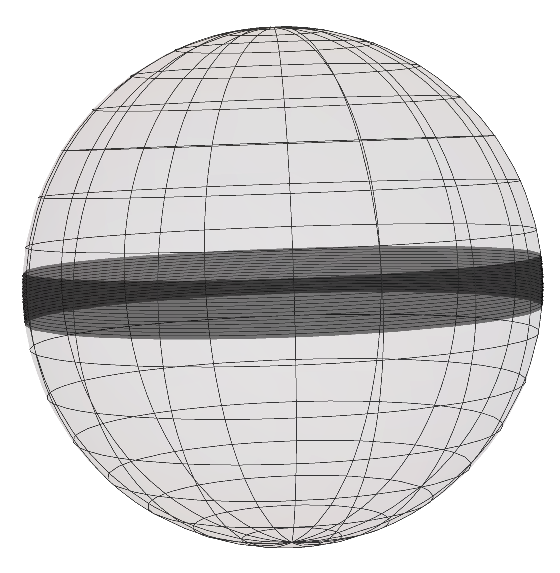
\includegraphics[scale=0.35]{banda}
    \caption{The $\epsilon$-strip of $\mathbb{S}^2(1)$ is the $\epsilon$-fattening of the equator of $\mathbb{S}^2(1)$}
    \label{fig:e-strip}
\end{figure}
\end{center}

Then, the measure concentration around the equator $E$ can be stated as  follows: 

\begin{corollary}[Measure concentration around the equator $E$]\label{equator}Given the $\epsilon$-strip $\Omega_\epsilon$ around the equator $E$, we have that
$$
\frac{{\rm vol}\left(\Omega_\epsilon\right)}{{\rm vol}\left(\mathbb{S}^n(1)\right)}\geq 1-\sqrt{\frac{\pi}{2}}e^{-\epsilon^2\frac{n-1}{2}}
$$
 and hence, for $0<\epsilon<1$ we have
$$
\lim_{n\to \infty}\frac{{\rm vol}\left(\Omega_\epsilon\right)}{{\rm vol}\left(\mathbb{S}^n(1)\right)}=1
$$
\end{corollary}

This Corollary \ref{equator} comes from the concentration of measure stated in Theorem \ref{measurecon} in the following way: let us denote as $\mathbb{S}^{n+}$ the half sphere centered at the north pole and  as $\mathbb{S}^{n-}$ the half sphere centered at the south pole. Then, the $\epsilon$-strip around the equator can be expressed, in terms of the $\epsilon$-fattening $\mathbb{S}^{n+}_{\epsilon}$ and $\mathbb{S}^{n-}_{\epsilon}$ as
$$\Omega_\epsilon=\mathbb{S}^{n+}_{\epsilon} \cap\mathbb{S}^{n-}_{\epsilon} $$
where the domains $A^+=\mathbb{S}^{n+}$ and $A^-= \mathbb{S}^{n-}$ concentrates measure in the Sphere in the sense of the above Theorem \ref{measurecon}. On the other hand, as ${\rm vol}(\mathbb{S}^{n+}_\epsilon)={\rm vol}(\mathbb{S}^{n-}_\epsilon)$, and by applying Theorem \ref{measurecon} to the domain $A^+=\mathbb{S}^{n+}$, we have that 
$$
\begin{aligned}
    \frac{{\rm vol}\left(\Omega_\epsilon\right)}{{\rm vol}\left(\mathbb{S}^n(1)\right)}=&
2\left(\frac{{\rm vol}(\mathbb{S}^{n+}_{\epsilon} )}{{\rm vol}(\mathbb{S}^n(1))}-\frac{1}{2}\right)\geq 2\left( 1-\sqrt{\frac{\pi}{8}}e^{-\epsilon^2(n-1)/2}-\frac{1}{2}\right)\\
=&1-\sqrt{\frac{\pi}{2}}e^{-\epsilon^2\frac{n-1}{2}}.
\end{aligned}
$$
\begin{figure}
    \centering
    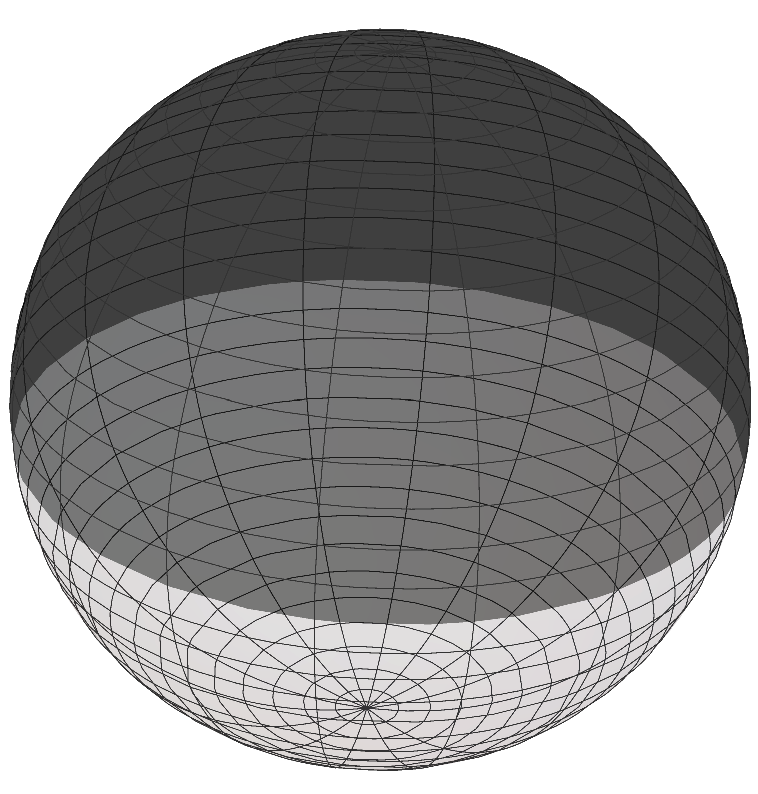
\includegraphics[scale=0.25]{positiva}\quad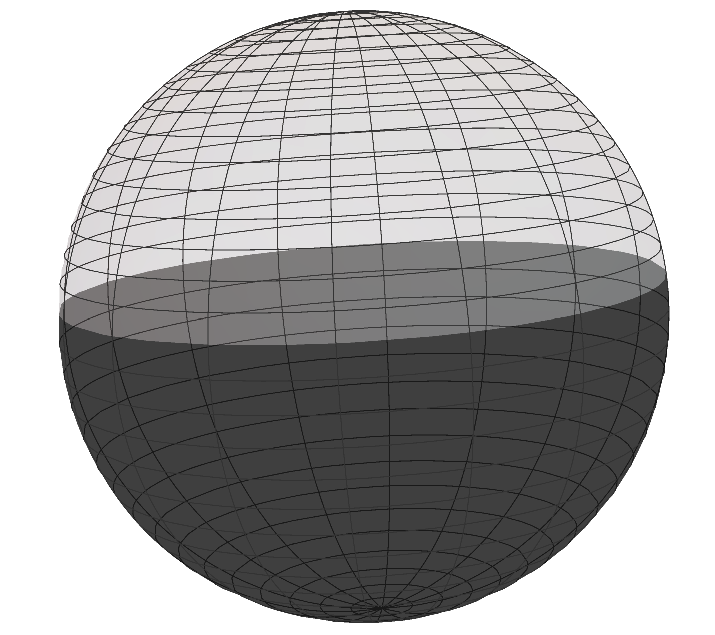
\includegraphics[scale=0.3]{negativa}
    \caption{The $\epsilon$-strip is the intersection between the $\epsilon$-fattening of the north hemisphere $\mathbb{S}^{+}_\epsilon$ and the $\epsilon$-fattening of the north hemisphere $\mathbb{S}^{-}_\epsilon$.}
    \label{fig:asintersection}
\end{figure}
The conclusion is that for  \lq\lq very large'' dimension,  almost all measure in the Sphere is concentrated surrounding  the equator. 

\begin{remark}
 We would like to draw attention to the following observation, which only apparently constitutes a paradox that would refute the last Corollary: let us consider an small $\epsilon >0$. Then, by virtue of Corollary \ref{equator}, as the dimension increases, the equatorial band occupies more and more area of the sphere, so that the two complementary big caps to the band have a small volume compared to the total volume of the sphere. 
 
 Let us now consider a rotation of the equatorial strip, (an isometry of the sphere acting on the strip), in such a way that the image due to this rotation of the strip is a domain in the sphere that cuts the two previous big caps. Since the image by the isometry of the band is a domain with the same area as the band and it occupies a large amount of area of the sphere, all this area will be concentrated outside the intersection with the caps, (which have small area). 
  The conclusion is that the entire area of the band will be concentrated in two small squares, antipodal and disconnected, which are the result of intersecting the old band prior to the rotation with the new one, (see picture below).
 \begin{figure}
     \centering
     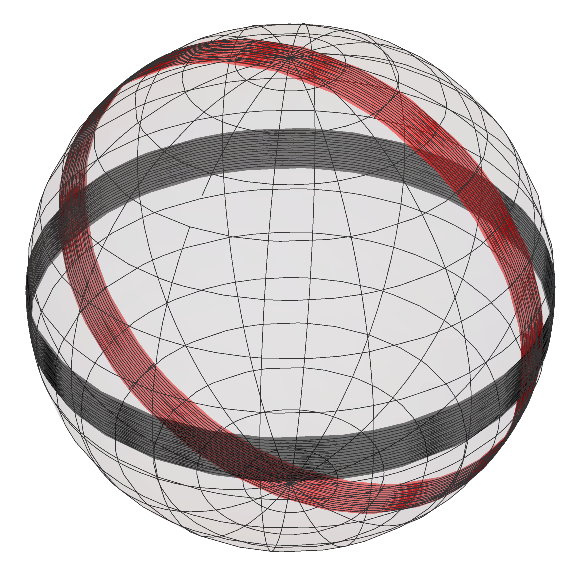
\includegraphics[scale=0.3]{dosbandes}
     \caption{Caption}
     \label{fig:enter-label}
 \end{figure}
 \begin{center}
\end{center}
 This fact not only does not contradict the corollary, but we must observe that, if we take, within one of these small squares, a spherical cap centered on it and circumscribed in it, we have that, when the dimension tends to infinity, the volume of this cap tends to zero while the area of the square tends to infinity.
\end{remark}

We use this last \lq\lq equatorial" measure concentration to introduce the notion of  {\em extrinsic equatorial concentration of measure}  of the submanifold $\Sigma \subseteq \mathbb{S}^n(1)$. 

Let us consider $x: \Sigma^m \to \mathbb{S}^n(1)$ be a complete isometric immersion of the  $m$-dimensional manifold $\Sigma^m$ in the sphere. Any totally geodesic equator $\mathbb{S}^{n-1}(1)$ on a sphere  $\mathbb{S}^n(1)$ can be described in terms of the intrinsic distance of its points to a given fixed point $p$, (and, in this sense, the equator $E$ that has served above to exemplify the phenomenon of concentration of the equatorial measure, is the set of points that are distant from the north pole by a distance equal to $\frac{\pi}{2}$). This description is given in the following way: given a point $p \in \mathbb{S}^n(1)$, \emph{the equator of $\mathbb{S}^n(1)$ with respect to $p$} is defined as 
   
 $$
    %\begin{aligned}
E(p):=\left\{x=(x_1,\cdots,x_{n+1})\in \mathbb{S}^n(1)\, :\,\,{\rm dist}^{\mathbb{S}^n(1)}(p,x)=\frac{\pi}{2} \right\},
%\end{aligned}
    $$
    where 
    $${\rm dist}^{\mathbb{S}^n(1)}(p,x)=\angle{(p,x)}=\arccos(p\cdot x)$$
    denotes the intrinsic distance in $\mathbb{S}^n(1)$ between the points $p$ and $x$.  Then,   \emph{the strip around the equator $E(p)$} is defined as the set:
    

$$
\begin{aligned}
\Omega(p,\epsilon)&=\left\lbrace x\in \mathbb{S}^{n}(1)\, : \, \frac{\pi}{2}-\epsilon<{\rm dist}^{\mathbb{S}^{n}(1)}(p,x)=\angle{(p,x)}<\frac{\pi}{2}+\epsilon\right\rbrace\\&=\left\lbrace x\in \mathbb{S}^{n}(1)\, : \,   \cos\left({\rm dist}^{\mathbb{S}^{n}(1)}(p,x)\right)\in ( -\sin\epsilon,\sin\epsilon) \right\rbrace.
\end{aligned}
$$

Our main result can be summarized asserting that there is an {\em extrinsic} equatorial concentration of measure when we consider minimal and compact submanifolds $\Sigma^m$ of any co-dimension in the Sphere $\mathbb{S}^n(1)$ and it is stated as follows:

\begin{theorem}
Let  $x: \Sigma^m \to \mathbb{S}^n(1)$ be an isometric and minimal immersion of the closed $m$-dimensional manifold $\Sigma$ in the sphere  $\mathbb{S}^n(1)$. Then, for any point $p \in \mathbb{S}^n(1)$ and any  $\epsilon \in (0,\pi/2)$ we have 

$$
1\geq \frac{{\rm vol}\left(x^{-1}(\Omega(p,\epsilon))\right)}{{\rm vol}(\Sigma)}\geq  1- \sqrt{2}e^{-\bar\epsilon^2(m+1)/4}
$$
where $\bar\epsilon=\sin\epsilon \in (0,1)$. Hence, for each  $\epsilon$,
$$
\lim_{m\to\infty}\frac{{\rm vol}\left(x^{-1}(\Omega(p,\epsilon))\right)}{{\rm vol}(\Sigma)}=1.
$$


\end{theorem}

\begin{remark}\

\begin{enumerate}
\item In this extrinsic case, the proof is based on the divergence theorem, (rather than on the isoperimetric inequality, as occurs in the intrinsic case).

\item We can recover the {\em intrinsic} equatorial concentration of measure as a corollary of the {\em extrinsic} equatorial  concentration of measure, taking $\Sigma=\mathbb{S}^n(1)$. In fact, if $\Sigma=\mathbb{S}^n(1)$, then we can use $x$ as the identity map  and hence, 
$$x^{-1}(\Omega(p,\epsilon))=x(\Sigma) \cap \Omega(p,\epsilon) =\Omega(p,\epsilon)$$so
$$
\lim_{n\to\infty}\frac{{\rm vol}\left(x^{-1}(\Omega(p,\epsilon))\right)}{{\rm vol}(\mathbb{S}^n(1))}=\lim_{n\to\infty}\frac{{\rm vol}\left(\Omega(p,\epsilon)\right)}{{\rm vol}(\mathbb{S}^n(1))}=1
$$

\item  It should rest open the statement of an {\em intrinsic} concentration of measure for compact and minimal submanifolds of the sphere, namely, if $A \subseteq \Sigma$ is a domain with ${\rm vol}(A) \geq \frac{1}{2} {\rm vol}(\Sigma)$, then the $\epsilon$-fattening of $A$ in $\Sigma$ satisfies the inequality
\begin{equation*}
1 \geq \frac{{\rm vol}(A_\epsilon)}{{\rm vol}(\Sigma)}\geq 1-\sqrt{\frac{\pi}{8}}e^{-\epsilon^2(m-1)/2}
\end{equation*}
\noindent and hence, for all $\epsilon \in [0,\frac{\pi}{2}]$, 
\begin{equation*}
\lim_{m\to \infty} \frac{{\rm vol}(A_\epsilon)}{{\rm vol}(\Sigma)}= 1
\end{equation*}
 

Here, the $\epsilon$-fattening of $A$ in $\Sigma$ should be defined as
$$A_\epsilon:=\left\{x\in \Sigma\, :\, {\rm dist}^{\Sigma}(x,A)<\epsilon\, \right\}
$$

\end{enumerate}
\end{remark}



%%%%%%%%%%%%%%%%%
% \subsection{Outline}
%%%%%%%%%%%%%%%%%
\subsection{Outline}\

The structure of the paper can be outlined as follows: after this Introduction where the notions related with the intrinsic and extrinsic equatorial concentration in the sphere has been presented, as well as a first glimpse of our main result, we shall follow in the following Section \S.2 with the study of the relative position of the closed and minimal submanifolds in the sphere with respect the equators of this sphere, proving a two-piece property which is satisfied by these closed and minimal submanifolds. Finally, we shall state and prove our main theorem in Section \S.3


%%%%%%%%%%%%%%%%%
% \subsection{Acknowledgement}
%%%%%%%%%%%%%%%%%
%\subsection{Acknowledgement}\

%The authors  wish to thank...


%%%%%%%%%%%%%%%%%%
%Section: Preliminaires
%%%%%%%%%%%%%%%%%%%%
\section{A high-dimensional two-piece property for parabolic and minimal submanifolds of the sphere $\mathbb{S}^n(1)$ }\

%%%%%%%%%%%%%%%%%%%%%%%%%%%%%%
%\subsection{Equator of a Sphere with respect a point}\
%%%%%%%%%%%%%%%%%%%%%%%%%%%%%%
%\medskip

We start with the definition of the {\em equator with respect a point} in the sphere $\ese^n(1)$, and the {\em strip around an equator }.

\begin{definition}
Given a point $p \in \mathbb{S}^n(1)$, \emph{the equator of  $\mathbb{S}^n(1)$ with respect to $p$} is defined as 
   
  $$
    \begin{aligned}
E(p):&=\left\{x=(x_1,\cdots,x_{n+1})\in \mathbb{S}^n(1)\, :\,\,{\rm dist}^{\mathbb{S}^n(1)}(p,x)=\frac{\pi}{2} \right\}\\&=
\left\{(x_1,\cdots,x_{n+1})\in \mathbb{S}^n(1)\, : \,\,\, p_1x_1+\cdots+p_{n+1}x_{n+1}=0\right\}
\end{aligned}
    $$
    \end{definition}
    
    In its turn, the {\em strip around an equator } is defined as:
    
\begin{definition}
The strip around the equator $E(p)$ is defined as the set:
    $$
\begin{aligned}
\Omega(p,\epsilon)&=\left\lbrace x\in \mathbb{S}^{n}(1)\, : \, \frac{\pi}{2}-\epsilon<{\rm dist}^{\mathbb{S}^{n}(1)}(p,x)=\angle{(p,x)}<\frac{\pi}{2}+\epsilon\right\rbrace\\&=\left\lbrace x\in \mathbb{S}^{n}(1)\, : \,   \cos\left({\rm dist}^{\mathbb{S}^{n}(1)}(p,x)\right)\in ( -\sin\epsilon,\sin\epsilon) \right\rbrace
\end{aligned}
$$
Hence, as $\epsilon \in (0,\frac{\pi}{2})$, if we put $\bar \epsilon=\sin \epsilon \in (0,1)$, then
$$
\Omega(p,\epsilon) =\left\lbrace x\in \mathbb{S}^{n}(1)\, : \, -\bar \epsilon<\cos\left({\rm dist}^{\mathbb{S}^{n}(1)}(p,x)\right)<\bar \epsilon\right\rbrace.
$$
\end{definition}

With these definitions at hand, it is evident that for any point $q\in E(p)$, 
        $$
{\rm dist}^{\mathbb{S}^n(1)}(p,q)=\frac{\pi}{2}={\rm dist}^{\mathbb{S}^n(1)}(-p,q)
        $$
where $-p$ denotes the antipodal point of $p \in \mathbb{S}^{n}(1)$. It is also evident  that any equator in the sphere $\mathbb{S}^n(1)$ is an equator with respect to some $p$.
        
     Let us consider now $x: \Sigma^m \to \mathbb{S}^n(1)$  a complete isometric immersion of the  $m$-dimensional manifold $\Sigma^m$ in the sphere.  A natural question that arises in this context is to ask ourselves about the position of the submanifold with respect to the equators of the ambient sphere. 
     
     In fact, when $\Sigma=\mathbb{S}^{1}(1)$ is a great circle isometrically immersed in the sphere $\mathbb{S}^{2}(1)$, it is not hard to show that then $\Sigma$ intersects {\em all} the equators of $ \mathbb{S}^{2}(1)$, (which are the great circles of the $2$-dimensional sphere).
     
     When the dimension of the ambient sphere is $3$, A. Ros showed in \cite{R} the following {\em Two-piece property}, which implies a more general intersection result to that described above for the two-dimensional case. In fact, every equator of the 3-sphere $\mathbb{S}^3(1)$ divides each embedded closed (compact, without boundary) non-totally geodesic minimal surface in exactly two open connected pieces.
     
    
  Therefore,  a natural question which arises in this context is following: under what conditions, (topological, analytical, curvature restrictions, etc), it is guaranteed, (for any dimension of the ambient sphere and any co-dimension of the immersed submanifold), that the submanifold cuts all the equators of the ambient sphere, namely
        $$x(\Sigma) \cap E(p) \neq \emptyset\,\,\,\forall p \in \mathbb{S}^n(1)$$ and hence, will intersect all the $\epsilon$-strips
        $$x(\Sigma) \cap \Omega(p,\epsilon) \neq \emptyset?, (\text{i.e.}, x^{-1}(\Omega(p,\epsilon))\neq \emptyset\,\,\,\forall p \in \mathbb{S}^n(1))$$
   
    Our first result describes  the position of the submanifold with respect the equators of $\mathbb{S}^n(1)$ and their strips, when the submanifold is connected and parabolic and takes the form of a kind of a high dimensional two-piece property:
 
\begin{theorem}\label{twopiecegeneral}

Let $x:\Sigma^m \to \mathbb{S}^n(1)$ be a complete,  minimal and isometric immersion, and let $p$ be any point of $\mathbb{S}^n(1)$. Suppose that $\Sigma$ is parabolic. Then
    \begin{itemize}
        \item Either $x(\Sigma)\subseteq E(p)$, 
        \item or, $x(\Sigma)\cap E(p)\neq \emptyset$
            \end{itemize}
            and  hence, in any case,  $x(\Sigma) \cap \Omega(p,\epsilon) \neq \emptyset$, ($x^{-1}(\Omega(p,\epsilon))\neq \emptyset$).
\end{theorem}

\begin{proof}
Let $K$ be a connected component of $\Sigma$. Since $\Sigma$ is parabolic, $K$ is a parabolic manifold as well.
Given $p\in \mathbb{S}^n(1)$, the \emph{extrinsic distance function} with respect to $p$ is the function given by
$$
\begin{aligned}
r_p:K \to \mathbb{R}, \quad q\mapsto r_p(q):&={\rm dist}^{\mathbb{S}^n(1)}(p,x(q))\\&=\angle{(p,x(q))}=\arccos(p\cdot x(q))
\end{aligned}
$$
so, given $q \in K$, with $x(q)=(p_1,...,p_{n+1}) \in \mathbb{S}^n(1)$, we have that
$$
\cos(r_p(q))=p\cdot x(q) = p_1x_1+\cdots+p_{n+1}x_{n+1}
$$
 and hence, $\cos\circ r_p$ is smooth on $K$.   We need the following
\begin{lemma}\label{coslema}
Let $x:K^m \to \mathbb{S}^n(1)$ be a complete and minimal isometric immersion, and let $p$ be any point of $\mathbb{S}^n(1)$. Then, for all $q \in K$,
 \begin{equation}\label{cos}
%\begin{aligned}
\Delta^K \cos(r_p(q))=-m\cos(r_p(q))
%\end{aligned}
\end{equation}
\end{lemma}
\begin{proof}
  Applying Takahasi's Lemma, we have,  as $x$ is minimal, that 
  $$\Delta^K x_i=-m x_i\,\,\forall i=1,...,n+1$$
  so we conclude 
$$
\begin{aligned}
\Delta^K \cos(r_p(q))=&p_1\Delta^\Sigma x_1+\cdots+p_{n+1}\Delta^\Sigma x_{n+1}\\=&-m\left(p_1x_1+\cdots+p_{n+1}x_{n+1}\right)=-m\cos(r_p(q))
\end{aligned}
$$\end{proof}
To prove  the Theorem, first, let us observe that, if the extrinsic distance function is constant,
$\cos\circ r_p(q)=c \,\,\forall q \in \Sigma$, then 
$$0=\Delta^K \cos(r_p(q))=-m\cos\circ r_p(q)\,\forall q \in K,$$
so $r_p(q)=\frac{\pi}{2} \,\,\forall q \in \Sigma$ and hence, in this case we have that $$x(K) \subseteq E(p).$$

This implies that the extrinsic distance function is a constant function if and only if $x(K)\subseteq E(p)$.
Now,  let us suppose that $x(K) \not\subseteq E(p)$ and that $x(K)\cap  E(p)=\emptyset$. Then $\cos\circ r_p$ is not constant on $K$ and, moreover, as $K$ is connected,  if $x(K)\cap  E(p)=\emptyset$ then $r_p(q) \in [0,\frac{\pi}{2})\,\,\forall q \in K$ or $r_p(q) \in (\frac{\pi}{2},\pi]\,\,\forall q \in K$. To see this last assertion, let us note that, in case there are points $q_1, q_2 \in K$ such that $r_p(q_1) \in [0,\frac{\pi}{2})$ and  $r_p(q_2) \in (\frac{\pi}{2},\pi]$, then we can conclude that there are points $q_1, q_2 \in K$ such that $\cos(r_p(q_1)) >0$ and  $\cos (r_p(q_2)) <0$, and therefore, $K$ is not connected because $K=\{ q \in K: \cos(r_p(q)) >0\}\cup \{ q \in K: \cos(r_p(q))< 0\} $. We can conclude therefore that $\cos\circ r_p$ is a bounded non-constant subharmonic, (superharmonic), function defined on $K$, which is a contradiction with the parabolicity of $K$. Hence, if  $x(K) \not\subseteq E(p)$, then $x(K)\cap  E(p)\neq \emptyset$, which implies that $x(\Sigma)\cap  E(p)\neq \emptyset$.\end{proof}
Note that, given the compact, (and hence, parabolic), and minimal submanifold $\Sigma$, we can apply  the above theorem \ref{twopiecegeneral} to conclude the following corollary:
\begin{corollary}
	Let  $x: \Sigma^m \to \mathbb{S}^n(1)$ be an isometric and minimal immersion of a closed, (compact without boundary), $m$-dimensional manifold $\Sigma$ in the sphere  $\mathbb{S}^n(1)$, and let $p$ be any point of $\mathbb{S}^n(1)$.  Then
    \begin{itemize}
        \item Either $x(\Sigma)\subseteq E(p)$, 
        \item or, $x(\Sigma)\cap E(p)\neq \emptyset$
            \end{itemize}
            and  hence, in any case,  $x(\Sigma) \cap \Omega(p,\epsilon) \neq \emptyset$, ($x^{-1}(\Omega(p,\epsilon))\neq \emptyset$).
\end{corollary}
In conclusion, in this first result, we have seen that when $x: \Sigma^m \to \mathbb{S}^n(1)$ is  compact and minimal, then \emph{always} there are points of $x(\Sigma)$ included in any equatorial strip, some in one part of the equator, some in the other part.

%%%%%%%%%%%%%%%%%%
\section{Main result}
%%%%%%%%%%%%%%%%%%%%

In the above Section we have seen that when $x: \Sigma^m \to \mathbb{S}^n(1)$ is  compact and minimal, then \emph{always} there are points of $x(\Sigma)$ included in any equatorial strip, some in one part of the equator, some in the other part. The question now is to estimate the \lq\lq amount" of such points in $x(\Sigma)$ which are included in these equatorial strips. 

We shall see that, as occurs in the intrinsic case, as the dimension increases, the \lq\lq greater'' the number of points of the submanifold within the equatorial strips. Namely, we observe an \emph{ extrinsic measure concentration phenomenon} satisfied by $x: \Sigma\to \mathbb{S}^n(1)$.

These ideas are stated in the following results:

\begin{theorem}[Main I]\label{extrinsicconc1}
Let  $x: \Sigma^m \to \mathbb{S}^n(1)$ be an isometric and minimal immersion of the closed $m$-dimensional manifold $\Sigma$ in the sphere  $\mathbb{S}^n(1)$. Then, for any point $p \in \mathbb{S}^n(1)$ and any  $\epsilon \in (0,\pi/2)$ we have 

$$
 1 \geq \frac{{\rm vol}\left(x^{-1}(\Omega(p,\epsilon))\right)}{{\rm vol}(\Sigma)}\geq1-\frac{1}{(m+1)\sin^2\epsilon}.
$$ Hence, for each $p$ and $\epsilon$,
$$
\lim_{m\to\infty}\frac{{\rm vol}\left(x^{-1}(\Omega(p,\epsilon))\right)}{{\rm vol}(\Sigma)}=1.
$$
\end{theorem}
\begin{proof}\


Given the extrisic distance function $r_p: \Sigma \rightarrow \erre$, we know that

\begin{equation}\label{eqOne}
\begin{aligned}
\Div^\Sigma\big(\cos (r_p(q))\,\nabla^\Sigma \cos(r_p(q))\big)=&\cos(r_p(q))\big(\Delta^\Sigma\cos(r_p(q))\big)\\&+\Vert \nabla^\Sigma \cos(r_p(q))\Vert^2.
\end{aligned}
\end{equation}
Then, since $\Delta^\Sigma \cos(r_p(q))=-m\cos(r_p(q))$, and integrating equation \eqref{eqOne} along $\Sigma$, we have, using that $\Sigma$ is compact and the divergence theorem:

\begin{equation}\label{eq:longa}
    \begin{aligned}
m\int_\Sigma\cos^2(r_p)=&\int_\Sigma\Vert \nabla^{\Sigma}  \cos(r_p)\Vert^2-\int_\Sigma \Div^\Sigma\big(\cos(r_p)\nabla^\Sigma \cos(r_p)\big)\\
=&\int_\Sigma \sin^2(r_p)\Vert \nabla^{\Sigma} r_p\Vert^2\\\leq& \int_\Sigma \sin^2(r_p)
={\rm vol}(\Sigma)- \int_\Sigma \cos^2(r_p).
\end{aligned}
\end{equation}
Then
\begin{equation}\label{eq:nula}
(m+1)\int_\Sigma \cos^2(r_p)\leq {\rm vol}(\Sigma).    
\end{equation}
Which implies, as  $\Sigma-x^{-1}(\Omega(p,\epsilon)) \subseteq \Sigma$,
\begin{equation}\label{eq:unua}
(m+1)\int_{\Sigma-x^{-1}(\Omega(p,\epsilon))} \cos^2(r_p)\leq {\rm vol}(\Sigma)    
\end{equation}
The strip around the equator $E(p)$ is ($\bar \epsilon=\sin \epsilon$):
$$
\Omega(p,\epsilon) =\left\lbrace x\in \mathbb{S}^{n}(1)\, : \, -\bar \epsilon<\cos\left({\rm dist}^{\mathbb{S}^{n}(1)}(p,x)\right)<\bar \epsilon\right\rbrace.
$$
Since $r_p(q):={\rm dist}^{\mathbb{S}^{n}(1)}(p,x(q))$, the set $x^{-1}(\Omega(p,\epsilon))$ can be written as 
$$
x^{-1}(\Omega(p,\epsilon))=\left\lbrace q \in \Sigma\,:\, -\bar \epsilon<\cos\left(r_p(q))\right)<\bar \epsilon\right\rbrace.
$$ Then for all $q \in\Sigma-x^{-1}(\Omega(p,\epsilon))$, we have
$ \bar\epsilon^2 \leq \cos^2(r_p(q))$  and by using inequality \eqref{eq:unua} we conclude that
 $$
(m+1)\bar \epsilon^2\left({\rm vol}(\Sigma)-{\rm vol}(x^{-1}(\Omega(p,\epsilon)))\right)\leq {\rm vol}(\Sigma),
$$ which finally implies the statement of the Theorem:
$$
\frac{{\rm vol}(x^{-1}(\Omega(p,\epsilon)))}{{\rm vol}(\Sigma)}\geq 1-\frac{1}{(m+1)\bar\epsilon^2}.
$$\end{proof}


\begin{theorem}[Main II]\label{extconc2}
Let  $x: \Sigma^m \to \mathbb{S}^n(1)$ be an isometric and minimal immersion of the closed $m$-dimensional manifold $\Sigma$ in the sphere  $\mathbb{S}^n(1)$. Then, for any point $p \in \mathbb{S}^n(1)$ and any  $\epsilon \in (0,\pi/2)$ we have 

$$
1\geq \frac{{\rm vol}(x^{-1}(\Omega(p,\epsilon)))}{{\rm vol}(\Sigma)}\geq 1- \sqrt{2}e^{-\bar\epsilon^2(m+1)/4}
$$
where $\bar\epsilon=\sin\epsilon \in (0,1)$. Hence, for each $p$ and $\epsilon$,
$$
\lim_{m\to\infty}\frac{{\rm vol}\left(x^{-1}(\Omega(p,\epsilon))\right)}{{\rm vol}(\Sigma)}=1
$$
\end{theorem}
\begin{proof}\

We need the following 

\begin{lemma}
Let  $x: \Sigma^m \to \mathbb{S}^n(1)$ be an isometric and minimal immersion of the closed $m$-dimensional manifold $\Sigma$ in the sphere  $\mathbb{S}^n(1)$ and let $p\in \mathbb{S}^n(1)$. Then

\begin{equation}\label{lemmaformula1}
\int_\Sigma \cos^{2k}(r_p) \leq \frac{\int_{\mathbb{S}^m(1)} \cos^{2k}(\widetilde{r}_p)}{{\rm vol}(\mathbb{S}^m(1))} {\rm vol}(\Sigma)
\end{equation}
where  $\widetilde{x}: \mathbb{S}^m(1) \rightarrow \mathbb{S}^n(1)$ is a totally geodesic immersion of $\ese^m(1)$ in $\ese^n(1)$, $r_p$ is the extrinsic distance function to $p$ given bay $x$, and $\widetilde{r}_p$ is the extinsic distance to $p$ given by $\widetilde{x}$. As a consequence, we have the following inequality,  for a given $t>0$:

\begin{equation}\label{lemmaformula2}
%\begin{aligned}
\int_{\Sigma} e^{t \cos^2r_p}  \leq\frac{\int_{\ese^m(1)} e^{t \cos^2\widetilde{r}_p}}{{\rm vol}(\mathbb{S}^m(1))} {\rm vol}.(\Sigma)
%\end{aligned}
\end{equation}
\end{lemma}
\begin{proof}

Let us apply an inductive argument to prove inequality (\ref{lemmaformula1}): we are going to see first that this inequality is true for $k=1$.  From \eqref{eq:longa} using that $\Vert r_p\Vert\leq 1$ we conclude inequality \eqref{eq:nula}:
$$
\int_\Sigma \cos^2(r_p) \leq \frac{1}{m+1} {\rm vol}(\Sigma)
$$
Now, if we consider the totally geodesic submanifold $\widetilde{x}: \mathbb{S}^m(1) \rightarrow \mathbb{S}^n(1)$, similarly to \eqref{eq:longa} using that $\Vert\nabla^{\mathbb{S}^m(1)} \widetilde{r}_p\Vert=1$, because $\widetilde{x}$ is a totally geodesic immersion, we conclude the following equality
\begin{equation}\label{eqcinc}
\int_{\mathbb{S}^m(1)} \cos^2(\widetilde{r}_p) = \frac{1}{m+1} {\rm vol}(\mathbb{S}^m(1)).
\end{equation}

Hence,  we have 
\begin{equation}\label{eqsis}
\int_\Sigma \cos^2(r_p) \leq \frac{\int_{\mathbb{S}^m(1)} \cos^2(\widetilde{r}_p)}{{\rm vol}(\mathbb{S}^m(1))} {\rm vol}(\Sigma)
\end{equation}
and we have proved that the inequality (\ref{lemmaformula1}) is true for $k=1$.

Assuming that it is true for $k >1$, namely, that
\begin{equation}\label{eqsisBis}
\int_\Sigma \cos^{2k}(r_p) \leq \frac{\int_{\mathbb{S}^m(1)} \cos^{2k}(\widetilde{r}_p)}{{\rm vol}(\mathbb{S}^m(1))} {\rm vol}(\Sigma),
\end{equation}
we see that it holds for $k+1$ in the following way: by using lemma \ref{coslema}  we have  for any $q\in \Sigma$ that

\begin{equation}
\begin{aligned}
\Div^\Sigma\left(\cos^{2k+1} (r_p(q))\,\nabla^\Sigma \cos(r_p(q)\right)=&\cos^{2k+1}(r_p(q))\Delta^\Sigma\cos(r_p(q)\\&+(2k+1) \cos^{2k}(r_p(q))\Vert \nabla^\Sigma \cos(r_p(q))\Vert^2\\
=&-m\cos^{2k+2}(r_p(q))\\&+(2k+1) \cos^{2k}(r_p(q))\Vert \nabla^\Sigma \cos(r_p(q))\Vert^2.
\end{aligned}
\end{equation}
Then, integrating the above equation  along $\Sigma$, we have, using that $\Sigma$ is compact and the divergence theorem:

\begin{equation}\label{eqdossBis}
\begin{aligned}
m\int_\Sigma \cos^{2(k+1)}(r_p)=&(2k+1)\int_\Sigma\cos^{2k}(r_p)\Vert \nabla^{\Sigma}  \cos(r_p)\Vert^2\\&-\int_\Sigma \Div^\Sigma\left(\cos^{2k+1}(r_p))\nabla^\Sigma \cos(r_p)\right)
\\
=&(2k+1)\int_\Sigma \cos^{2k}(r_p)\sin^2(r_p)\Vert \nabla^{\Sigma} r_p\Vert^2\\
=&(2k+1)\int_\Sigma \cos^{2k}(r_p)\left(1-\cos^2(r_p)\right)\Vert \nabla^{\Sigma} r_p\Vert^2\\
\leq& (2k+1)\int_\Sigma \cos^{2k}(r_p)-(2k+1)\int_\Sigma \cos^{2k+2}(r_p).
\end{aligned}
\end{equation}
Thence
\begin{equation}\label{eqdoss2Bis}
\begin{aligned}
\int_\Sigma \cos^{2(k+1)}(r_p)\leq &\frac{2k+1}{m+2k+1}\int_\Sigma \cos^{2k}(r_p)\\ 
\leq&  \frac{2k+1}{m+2k+1}\frac{\int_{\mathbb{S}^m(1)} \cos^{2k}(\widetilde{r}_p)}{{\rm vol}(\mathbb{S}^m(1))} {\rm vol}(\Sigma)
\end{aligned}
\end{equation}

On the other hand, same computations than in (\ref{eqdossBis}), but when we consider the totally geodesic immersion of $\ese^m(1)$ in $\ese^n(1)$ gives the formula

$$
\begin{aligned}
m\int_{\ese^m(1)} \cos^{2(k+1)}(\widetilde{r}_p)=&(2k+1)\int_{\ese^m(1)}\cos^{2k}(\widetilde{r}_p)-(2k+1)\int_{\ese^m(1)} \cos^{2k+2}(\widetilde{r}_p)
\end{aligned}
$$
and hence
\begin{equation}\label{eqdoss4Bis}
%\begin{aligned}
\int_{\ese^m(1)} \cos^{2(k+1)}(\widetilde{r}_p)=\frac{2k+1}{m+2k+1}\int_{\ese^m(1)}\cos^{2k}(\widetilde{r}_p)
%\end{aligned}
\end{equation}
Finally, using (\ref{eqdoss2Bis}) and (\ref{eqdoss4Bis}) we obtain

\begin{equation}\label{eqdoss5Bis}
\begin{aligned}
\int_\Sigma \cos^{2(k+1)}(r_p)\leq& \frac{2k+1}{m+2k+1}\int_\Sigma \cos^{2k}(r_p)\\  \leq & \frac{2k+1}{m+2k+1}\frac{\int_{\mathbb{S}^m(1)} \cos^{2k}(\widetilde{r}_p)}{{\rm vol}(\mathbb{S}^m(1))} {\rm vol}(\Sigma)\\
=&\frac{\int_{\mathbb{S}^m(1)} \cos^{2(k+1)}(\widetilde{r}_p)}{{\rm vol}(\mathbb{S}^m(1))} {\rm vol}(\Sigma)
\end{aligned}
\end{equation}

Now, we are going to prove inequality (\ref{lemmaformula2}): given a fixed $t>0$, we have, applying inequality (\ref{lemmaformula1}) that

$$\int_\Sigma\frac{t^k \cos^{2k}(r_p)}{k!} \leq \frac{\int_{\mathbb{S}^m(1)}\frac{t^k \cos^{2k}(\widetilde{r}_p)}{k!}}{{\rm vol}(\mathbb{S}^m(1))} {\rm vol}(\Sigma)$$
 so, applying dominated convergence theorem and the power series expansion of the exponential function, we have, for a given $t>0$:
$$
\begin{aligned}
\int_{\Sigma} e^{t \cos^2r_p} =&\sum_{k=0}^\infty \int_\Sigma\frac{t^k \cos^{2k}(r_p)}{k!} \\
\leq& 
\sum_{k=0}^\infty \frac{\int_{\mathbb{S}^m(1)}\frac{t^k \cos^{2k}(\widetilde{r}_p)}{k!}}{{\rm vol}(\mathbb{S}^m(1))} {\rm vol}(\Sigma)=\frac{\int_{\ese^m(1)} e^{t \cos^2\widetilde{r}_p}}{{\rm vol}(\mathbb{S}^m(1))} {\rm vol}(\Sigma)
\end{aligned}
$$
\end{proof}
Now, as we have seen in the proof of theorem \ref{extrinsicconc1}
we have that for all  $q \in\Sigma-x^{-1}(\Omega(p,\epsilon))$, 
$$ \bar\epsilon^2 \leq \cos^2(r_p(q))$$
and hence, for every $t >0$, and for all $q \in \Sigma- x^{-1}(\Omega(p,\epsilon))$,
$$e^{t\bar\epsilon^2} \leq e^{t\cos^2(r_p(q))} $$

Therefore, using inequality (\ref{eqsis}), we conclude
 \begin{equation}\label{eqsisBis}
 \begin{aligned}
e^{t\bar\epsilon^2}&\int_{\Sigma-x^{-1}(\Omega(p,\epsilon))} 1\leq 
\int_{\Sigma-x^{-1}(\Omega(p,\epsilon))}e^{t \cos^2r_p}\\&\leq \int_\Sigma e^{t\cos^2r_p} \leq \frac{\int_{\mathbb{S}^m(1)}e^{t \cos^2\widetilde{r}_p}}{{\rm vol}(\mathbb{S}^m(1))} {\rm vol}(\Sigma)
\end{aligned}
\end{equation}
Then we can state that
\begin{equation}\label{preskauxlasta}
    1-\frac{{\rm vol}(x^{-1}(\Omega(p,\epsilon))}{{\rm vol}(\Sigma)}\leq e^{-t\bar\epsilon^2}\frac{\int_{\mathbb{S}^m(1)}e^{t \cos^2\widetilde{r}_p}}{{\rm vol}(\mathbb{S}^m(1))}.
\end{equation}
Now we need the following 
\begin{lemma}\label{lastalemma} For any $0<t<\frac{m+1}{2}$,
$$
  \frac{\int_{\mathbb{S}^m(1)}e^{t \cos^2\widetilde{r}_p}}{{\rm vol}(\mathbb{S}^m(1))}\leq \sqrt{\frac{m+1}{m+1-2t}}.
    $$
\end{lemma}
\begin{proof}
    Let us define the function 
    $$
s\mapsto F(s):= \frac{\int_{\mathbb{S}^m(1)}e^{s \cos^2\widetilde{r}_p}}{{\rm vol}(\mathbb{S}^m(1))}.
    $$
  By the dominated convergence theorem we know that $F(0)=1$ and
     
    $$
F'(s)=\frac{\int_{\mathbb{S}^m(1)}\cos^2\widetilde{r}_pe^{s \cos^2\widetilde{r}_p}}{{\rm vol}(\mathbb{S}^m(1))}
    $$
 By using lemma \ref{coslema}, the divergence theorem, and that since the immersion is totally geodesic $\Vert \nabla\widetilde{r}_p\Vert^2=1$ we have 
 $$
\begin{aligned}
mF'(s)=&\frac{-\int_{\mathbb{S}^m(1)}\cos\widetilde{r}_pe^{s \cos^2\widetilde{r}_p}\Delta \cos\widetilde{r}_p}{{\rm vol}(\mathbb{S}^m(1))}
=\frac{-\int_{\mathbb{S}^m(1)}{\rm div}\left(\cos\widetilde{r}_pe^{s \cos^2\widetilde{r}_p}\nabla \cos\widetilde{r}_p\right)}{{\rm vol}(\mathbb{S}^m(1))}\\&+\frac{\int_{\mathbb{S}^m(1)}\left\langle\nabla \left(\cos\widetilde{r}_pe^{s \cos^2\widetilde{r}_p}\right),\nabla \cos\widetilde{r}_p\right\rangle}{{\rm vol}(\mathbb{S}^m(1))}\\
=&\frac{\int_{\mathbb{S}^m(1)}\sin^2\widetilde{r}_pe^{s \cos^2\widetilde{r}_p}}{{\rm vol}(\mathbb{S}^m(1))}+2s\frac{\int_{\mathbb{S}^m(1)}\sin^2\widetilde{r}_p{ \cos^2\widetilde{r}_p}e^{s \cos^2\widetilde{r}_p}}{{\rm vol}(\mathbb{S}^m(1))}\\
=&\frac{\int_{\mathbb{S}^m(1)}e^{s \cos^2\widetilde{r}_p}}{{\rm vol}(\mathbb{S}^m(1))}-\frac{\int_{\mathbb{S}^m(1)}\cos^2\widetilde{r}_pe^{s \cos^2\widetilde{r}_p}}{{\rm vol}(\mathbb{S}^m(1))}+2s\frac{\int_{\mathbb{S}^m(1)}\sin^2\widetilde{r}_p{ \cos^2\widetilde{r}_p}e^{s \cos^2\widetilde{r}_p}}{{\rm vol}(\mathbb{S}^m(1))}\\
\leq & F(s)-F'(s)+2sF'(s).
    \end{aligned}
 $$
 Thence, for $s<\frac{m+1}{2}$,
 $$
\frac{F'(s)}{F(s)}\leq \frac{1}{m+1-2s}
 $$
 Integrating the above inequality between $0$ and $t$ we conclude that
 $$
\ln F(t)\leq \ln \sqrt{\frac{m+1}{m+1-2t}}.
 $$
 and the lemma is proved.
\end{proof}
Taking now $t=\frac{m+1}{2\alpha}$ with $\alpha>1$, the above lemma and inequality \eqref{preskauxlasta} we conclude that
\begin{equation}\label{lasta}
     1-\frac{{\rm vol}(x^{-1}(\Omega(p,\epsilon))}{{\rm vol}(\Sigma)}\leq e^{-\bar\epsilon^2\frac{m+1}{2\alpha}}\sqrt{\frac{\alpha}{\alpha-1}}.
\end{equation}
Taking $\alpha=2$ the theorem is proved.\end{proof}
\begin{remark}
    From the proof of theorem \ref{extconc2} other versions with other constants. Observe that from \eqref{lasta} we can  state that for any $\delta>0$, the rhythm of growth of $\frac{{\rm vol}(x^{-1}(\Omega(p,\epsilon))}{{\rm vol}(\Sigma)}$ with respect to  the dimension $m$ is bounded from below by
    $$
    \frac{{\rm vol}(x^{-1}(\Omega(p,\epsilon))}{{\rm vol}(\Sigma)}\geq 1-e^{-\bar\epsilon^2\frac{m+1}{2+2\delta}}\sqrt{1+\frac{1}{\delta}}.
    $$
    Theorem \ref{extconc2} is obtained therefore by the particular choose of $\delta=1$ . But for any $\delta\in (0,1)$  we will obtain an improved growth of $\frac{{\rm vol}(x^{-1}(\Omega(p,\epsilon))}{{\rm vol}(\Sigma)}$ with respect to  the dimension $m$. Moreover, for  $m$ large enough we can assume that $\bar \epsilon^2>\frac{1}{m+1}$ (as in theorem \ref{extrinsicconc1}) and by choosing
    $$
    \delta=\frac{1}{\bar\epsilon^2(m+1)-1},
    $$
    We would obtain the improved bound
$$
    \frac{{\rm vol}(x^{-1}(\Omega(p,\epsilon))}{{\rm vol}(\Sigma)}\geq 1-\bar \epsilon \cdot e^{-\bar\epsilon^2\frac{m+1}{2}}\sqrt{e(m+1)}.
    $$
    This two bounds lead us to conjecture the following bound 
    $$
    \frac{{\rm vol}(x^{-1}(\Omega(p,\epsilon))}{{\rm vol}(\Sigma)}\geq 1-C e^{-\epsilon^2\frac{m-1}{2}},
    $$
    for some absolute constant $C>0$, in agreement with the intrinsic case.
\end{remark}


%%%%%%%%%%%%%%%%%%%%%%%%%%%%%%%%%%%%%
%%%%%%%%%%%%%%%%%%%%%%%%%%%%%%%%%%%%%

  %%%%%%%%%%%%%%%%
\begin{thebibliography}{10}
%%%%%%%%%%%%%%%%%%%
  


%\bibitem[GreW]{GreW} R. Greene and H. Wu,
%\textit{Function theory on manifolds which possess a pole}, Lecture Notes in
%Math., vol. 699, Springer-Verlag, Berlin and New York (1979).

   
%\bibitem[Gri3]{Gri3} A. Grigor'yan, \textit{Heat kernel and analysis on manifolds},  volume 47 of {\em AMS/IP studies in Advanced Mathematics},  Amer. Math. Soc., Providence, RI; International Press, Boston, MA, (2009).

%\bibitem[HS]{HS} R. Hardt and L. Simon, \textit{Nodal sets for solutions of elliptic equations}, J. Differential Geom.,
%\textbf{30}(2) (1989), 505--522.


\bibitem[MS]{MS} V. D. Milman and G. Schechtman,
\textit{Asymptotic Theory of Finite Dimensional Normed Spaces, with and Appendix by M. Gromov}, 2nd Printing,
Lecture Notes in Mathematics, \textbf{1200},  Springer Verlag,
Berlin (2001).

\bibitem[R]{R} A. Ros,
\textit{A Two-Piece Property for Compact Minimal Surfaces in a Three-Sphere}, Indiana University Mathematics Journal, \textbf{44}(3) (1995), 841--849

\bibitem[S]{S} T. Sakai, \textit{Riemannian Geometry}, Translations
of Mathematical Monographs Volume 149, American Mathematical
Society, 1996.


\end{thebibliography}



\end{document}


